\documentclass[../thesis.tex]{subfiles}

% graphics path
\graphicspath{
  {../../figures/chapter4/}
}

\begin{document}
\chapter{Preferential Pathways And Vapor Intrusion}

\begin{abstract}
Preferential pathways have recently been recognized for the significant role that they may play in enhancing exposure after their discovery at some well-studied VI sites.
The nature and specific effect of a preferential pathway can vary greatly and is largely site specific; generalizing their impact is therefore difficult.
One of these well-studied sites in Layton, Utah however, has a preferential pathway that had a very significant impact, which offers us an opportunity to explore this case in detail.
Through our numerical model and data analysis we are able to reveal how the preferential pathway at this site both enhanced the contaminant availability and advective potential which caused its significant impact.
We also examine the impact of the preferential pathway at another well-studied site in Indianapolis, Indiana, and compare that case to the one in Layton, and show that for seemingly relatively similar conditions, a preferential pathway may have very different results.

\end{abstract}


\section{Introduction}

To formulate a mathematical description of VI, we consider a simple hypothetical VI scenario at steady-state and develop a three-dimensional model of this.
Consider a VI impacted house with a \SI{10}{\metre} by \SI{10}{\metre} foundation footprint with a basement whose foundation lies \SI{1}{\metre} below ground surface (bgs).
There is also a \SI{1}{\centi\metre} wide crack along the perimeter of the \SI{15}{\centi\metre} thick foundation slab, where all contaminant vapor entry into the house is assumed to occur.
Here we will consider the basement alone as the control volume for which the indoor contaminant concentration will be determined.
It is assumed to have a ceiling height of \SI{3}{\metre}, giving a total volume of \SI{300}{\metre\cubed}
and that contaminant vapors are expelled via air exchange with the exterior of the house; the air exchange rate with outdoor air is assumed to be \SI{0.5}{\per\hour}.\par

The contaminant source be the underlying groundwater, which is assumed to be \SI{4}{\metre} bgs, and it is infinitely and homogenously contaminated with TCE (we will normalize everything to this source concentration, so the value does not matter), i.e. the groundwater contaminant concentration does not change over time nor does it have any concentration gradients.
We will only consider contaminant transport in the portion of soil between the open ground surface and the groundwater interface - the \textit{vadose zone}.
This soil is assumed to be homogenous and consist only of \textit{sandy loam} type soil, i.e. there no soil layers, rocks, etc.
For now, we will assume that no contaminant sorption into/onto the soil occurs, but this phenomena will be explored in Chapter (TBD).% TODO: Sorption chapter reference
The house is assumed to be surrounded by open ground that extend \SI{10}{\metre} from the house wall.
Contaminant concentration in the atmosphere is assumed so low that is effectively zero, i.e. contaminant vapors that reach the ground surface are immediately infinitely diluted. \par

The house interior is assumed to be slightly depressurized relative to ambient due to the stack effect; the indoor/outdoor pressure difference is \SI{-5}{\pascal}
This induces an airflow from the ground surface, through the soil, and into the house via the foundation crack.
The airflow interacts with contaminant diffusion in the soil.
Figure \ref{fig:vi_scenario} shows a figure summarizing this VI scenario.\par

% TODO Add a basement to the picture
\begin{figure}
  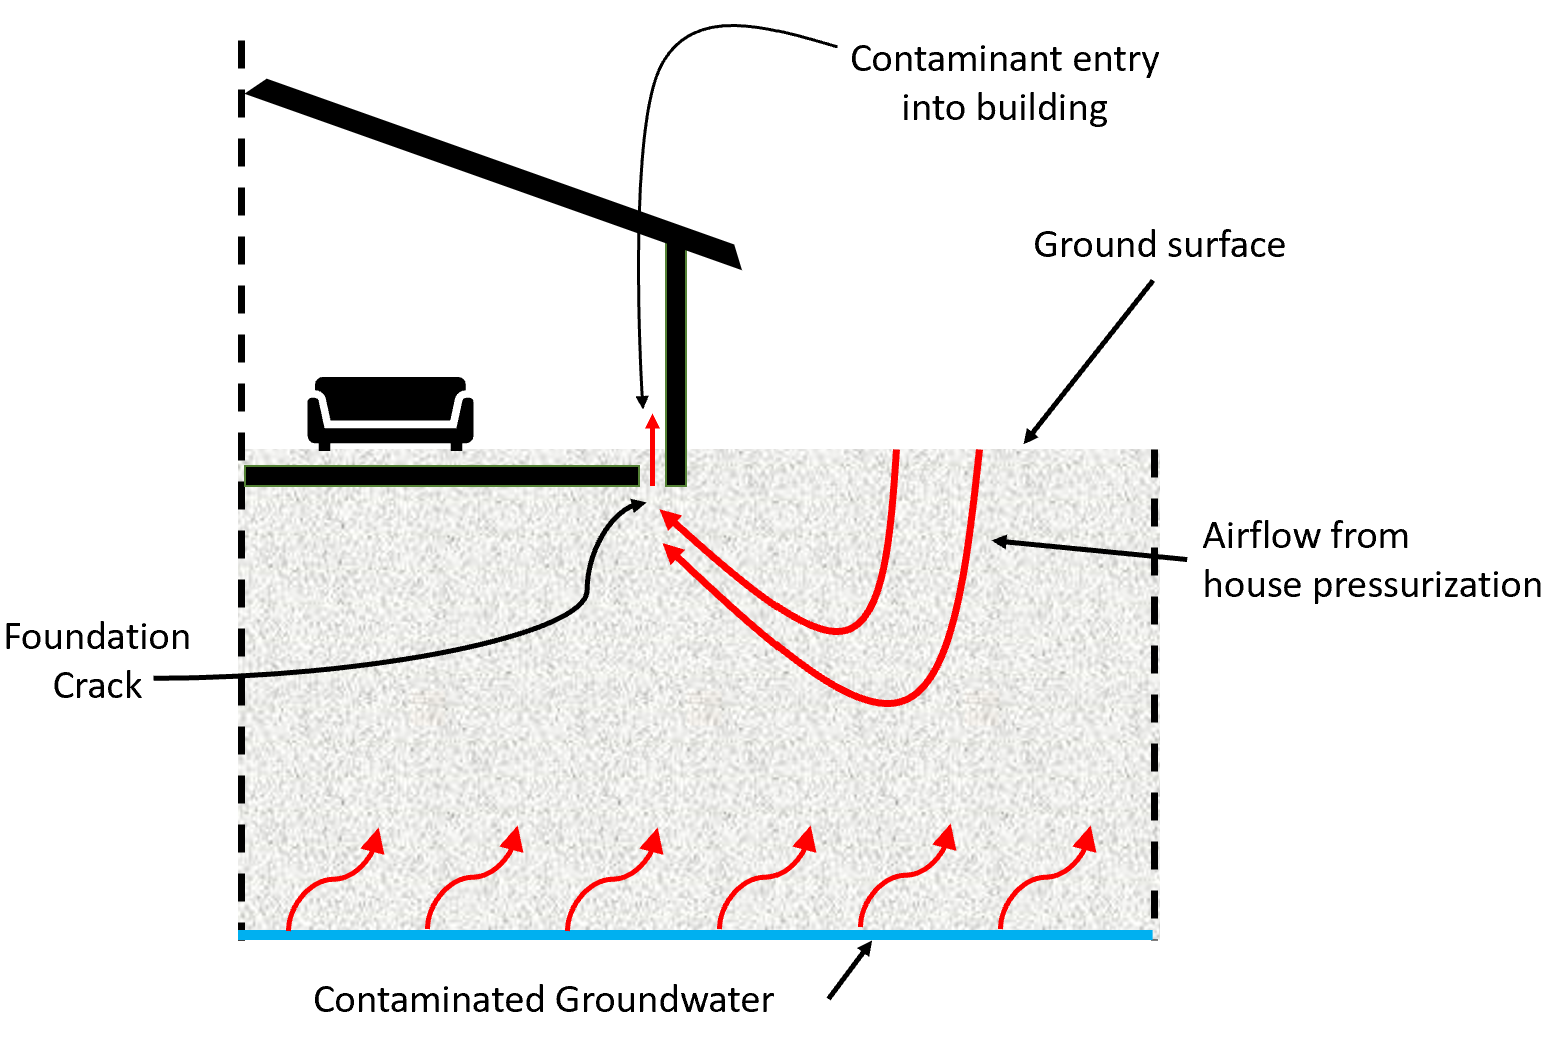
\includegraphics[width=\textwidth]{model_cartoon.png}
  \caption{The considered VI scenario.}
  \label{fig:vi_scenario}
\end{figure}

The basement interior will be modeled as a continuously stirred tank reactor (CSTR), (but without reactions), where the indoor contaminant concentration will depend on the contaminant entry rate $n_\mathrm{ck}$ from the soil via the foundation crack and the air exchange rate $A_e$.
The details of this will be covered section \ref{sec:indoor}.\par

To determine $n_\mathrm{ck}$ the contaminant transport in the soil needs to be modeled.
This will be done using the advection-diffusion equation, which will be modified for transport in soils.
The contaminant transport itself is driven by a concentration gradient and airflow in the soil.
The contaminant source (groundwater) and sink (atmosphere and contaminant entry into the building) will largely determine the concentration gradient, while the airflow needs to be calculated separately.\par

The airflow in the soil is modeled by Darcy's Law, and is driven by a pressure gradient in the soil, which induced by the indoor/outdoor pressure difference.
Details are in section \ref{sec:darcys_law}.\par

One last consideration is that the vadose zone is partially saturated with water, with the soil pores more or less filled near the groundwater interface, and with soil moisture content decreasing as a function of elevation above groundwater $z$ [\si{\metre}].
The soil moisture content has a profound effect on transport in the soil; it restricts both the airflow and contaminant diffusivity in the soil.
Thus, the soil moisture content $\theta_w$ must first be determined in order to solve the contaminant transport and Darcy's Law.\par

The resulting physical system is highly coupled, with many physical aspects dependant on others.
Figure \ref{fig:physics_overview} shows the coupling between each physicsal process, its output, and how it relates to the other processes that ultimately determine VI.\par

% TODO Add Millington-Quirk blob
\begin{figure}
  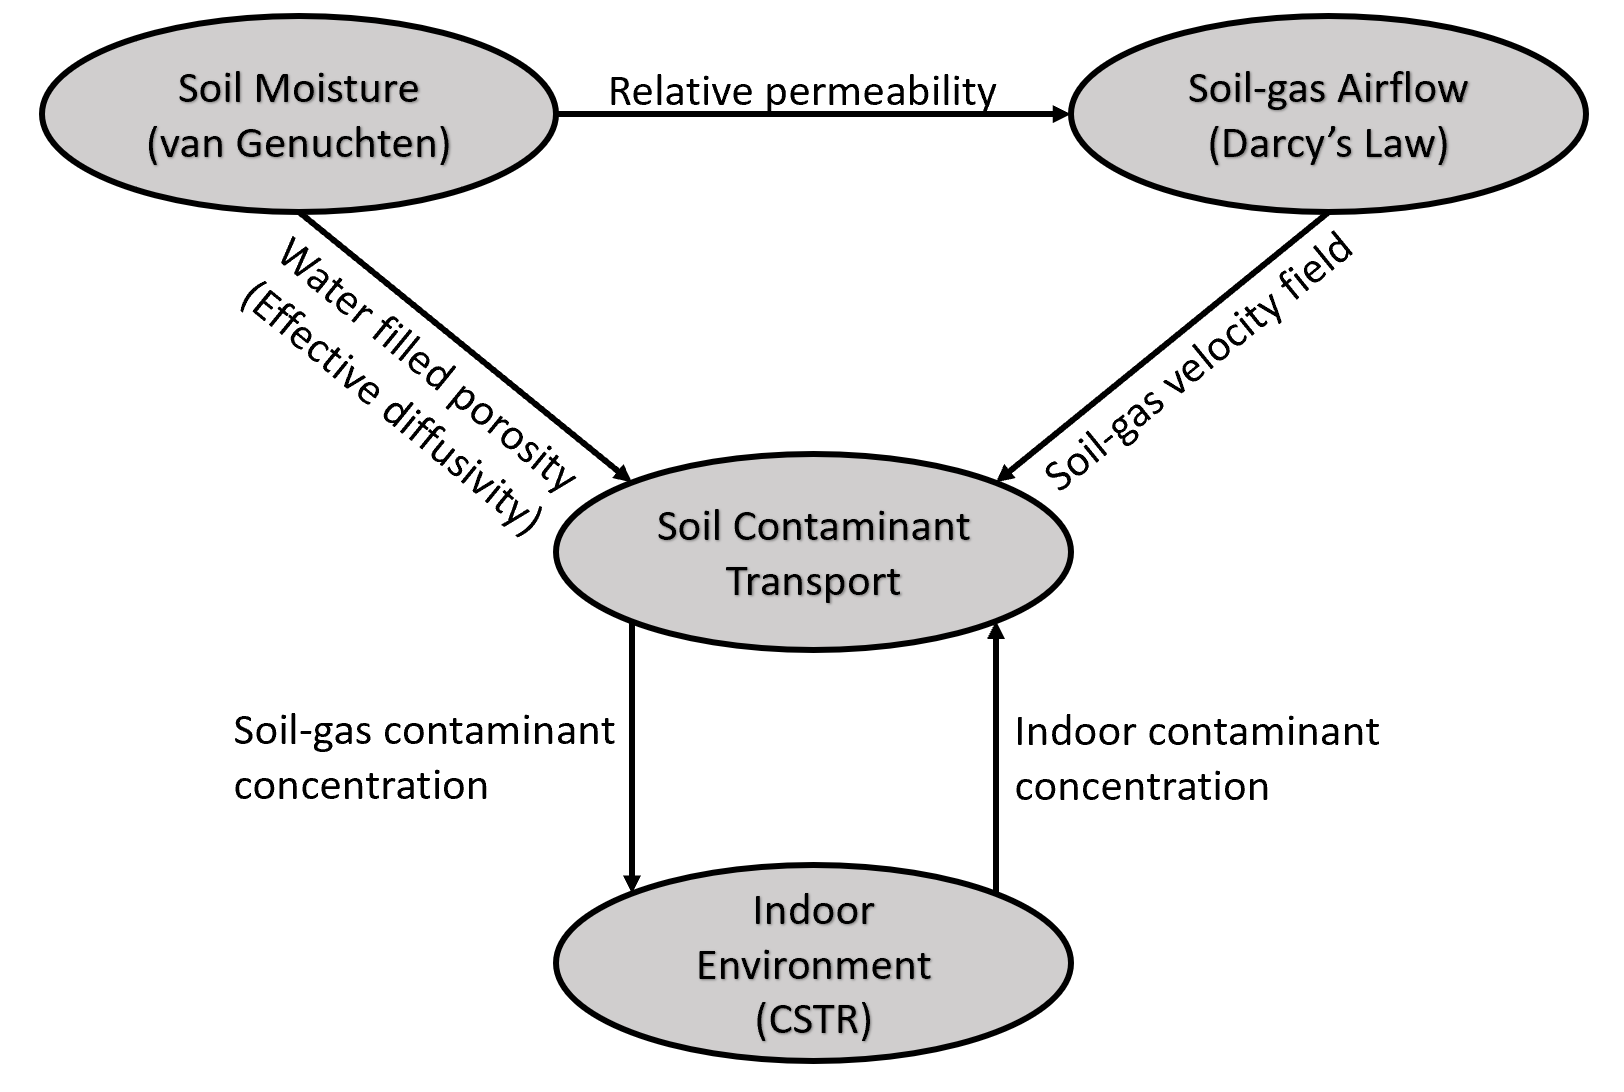
\includegraphics[width=\textwidth]{physics_interaction.png}
  \caption{Coupling between the physics used to model VI.}
  \label{fig:physics_overview}
\end{figure}

In this chapter, we will walk through the process of numerically modeling this VI scenario using the finite element method (FEM) and post-processing of the results.
A discussion regarding past and present VI models, their advantages and limitations, will follow.\par

\subsection{Finite Element Method}

% TODO Make it clear which sources I use here and say so early.
% TODO Make a figure showing the basis functions with nodal coefficients.

Many physical phenomena are described by partial differential equations (PDEs), but for anything but the simplest scenarios, these do not have an analytical closed-form solutions; therefore numerical methods are needed for finding an approximate solution.
This is achieved by discretizing the problem, i.e. transforming a continuous problem into a discrete one.
There are numerous ways to discretize a problem, and some of the more popular schemes are finite difference (FDM), finite volume (FVM), and finite element method (FEM).\par

In this work we use FEM, which is a popular numerical scheme that offers some distinct advantages over other schemes for modeling VI.
FEM subdivides the domain of the PDE problem into many smaller subdomains called elements.
These elements can take a wide variety of shapes, e.g. tetrahedra, prisms, or cuboids for three-dimensional problems and triangles or rectangles for two-dimensional problems.
The collection of elements that make up the domain or geometry is called a \textit{mesh}.
The fineness of the mesh is what largely determines the accuracy of the solution, but also increases the computational costs.\par

The size of each element can be highly nonuniform which allows FEM to discretize complicated geometries.
This is advantageous for modeling VI, where different parts of the geometry can have dramatically different resolution requirements; the \SI{1}{\centi\metre} foundation crack requires elements on the scale of \si{\milli\metre}, while in other parts of the geometry the resolution requirement is on the scale of \si{\metre}.
This ability to easily represent complicated geometries with elements of ununiform sizes helps maintain accuracy while saving computational resources.
Another benefit of using these elements is that it is easy to assign different constant values throughout the domain, and heterogenous materials can easily be represented.\par

The purpose of this work is not to provide a detailed description of the FEM, but for the interested reader \citeauthor{larson_finite_2010}\cite{larson_finite_2010} is a good resource.
However, it is important to know that FEM assumes that the approximated solution to a PDE can be written as a series of linear functions, called \textit{basis functions}.
\begin{equation}
  u \approx u_h = \sum^i u_i \psi_i
\end{equation}
here $u$ is the exact solution to the problem;
$u_h$ is the approximate solution;
$u_i$ is a \textit{nodal coefficient};
and $\psi$ is a \textit{basis function}.
These basis functions are usually some simple function, e.g. a hat function or some lower-order polynomial.\par

These basis functions are used to discretize the problem by rewriting a PDE into its \textit{weak form}, multiplying the equation with another set of functions called a \textit{test function}.
The test functions are the same type of function as the basis function, i.e. if the basis function is a hat function, so is the test function.
The result of this is an integral, where the integrands are the product of the basis function.
These integrals are numerically solved using some quadrature method, which gives a linear system of equations.
This system of equations is then solved to give all of the $u_i$ coefficients and thus the approximated solution $u_h$.\par

The point of this is that choice of basis function, i.e. hat function, first or third order polynomial, can influence the accuracy of the solution, and certain basis functions are more appropriate for certain PDEs.
Generally, higher order polynomials will give a more accurate solution, but at a computational cost, making it sometimes difficult to choose.
This adds another level of complexity of using FEM over some other numerical schemes, as the accuracy of the solution is not only influenced by the mesh but also somewhat by the choice of basis functions.
This highlights one of the drawbacks of FEM, i.e. that it is mathematically more challenging to implement and use than some other numerical schemes may be.\par

Fortunately, due to the attractiveness of the method, many commercial FEM packages have developed which increases usability significantly.
In this work we will use such a package - COMSOL Multiphysics, where subsequent sections will cover the steps required to implement our VI model in COMSOL.
(Of course, this could easily be translated into use in another software package.)\par

In order, we will cover:
\begin{enumerate}
  \item Creation of a model geometry.
  \item Defining physics/governing equations, boundary, and initial conditions.
  \item Discretize/mesh the geometry.
  \item Solver configuration.
  \item Post-process the results.
\end{enumerate}



\begin{comment}

Main point of this chapter:

Demonstrate how and why subsurface preferential pathways can have such a significant effect on VI.

Outline:

Introduction:
* How did we come to find out about PP?
* Why should we care about them?
* How do they work?

Methods:
* How do we model the PP?

Results & Discussion:

* Show how the model predicts the VI at the ASU house. (Main case)
* Turn on and off the enhanced advective potential and contaminant availability to show their contributions.
* Some other factors that affect PP "performance" in the main case. I.e. effect of gravel sub-base.


Conclusion:
* PPs need to enhance advective transport and introduce extra contaminants to be impactful (plus other factors). How common place these combination of factors are determine the concern for PPs.
* Suggestions for how to deal/uncover PPs? Follow Danish recommendations. See if subsurface piping may be discovered a priori. Sample nearby manholes (likely to play some role). Might even use CPM.

\end{comment}

\end{document}
